% Technical diagrams for the IEEE paper
\usepackage{tikz}
\usetikzlibrary{shapes.geometric, arrows, positioning, calc, shadows, patterns}

% System Architecture Diagram
\begin{figure}[h]
\centering
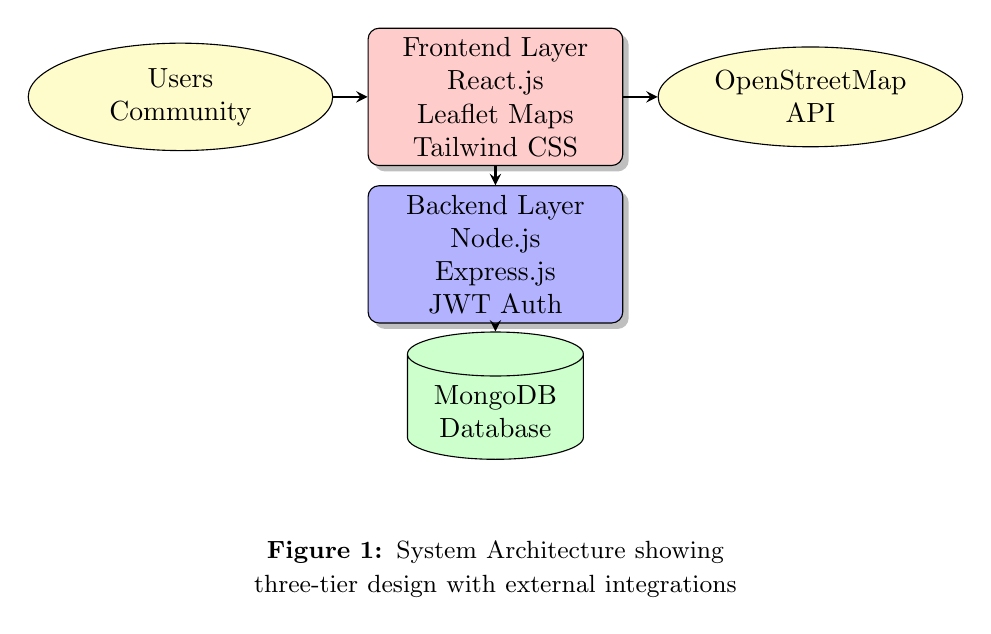
\begin{tikzpicture}[
    node distance=1.5cm,
    box/.style={rectangle, draw=black, fill=blue!20, text width=3cm, text centered, rounded corners, minimum height=1cm, drop shadow},
    arrow/.style={thick,->,>=stealth},
    database/.style={cylinder, draw=black, fill=green!20, shape border rotate=90, aspect=0.25, text width=2cm, text centered, minimum height=1.5cm},
    cloud/.style={ellipse, draw=black, fill=yellow!20, text width=2.5cm, text centered, minimum height=1cm}
]

% Frontend Layer
\node[box, fill=red!20] (frontend) at (0,4) {Frontend Layer\\React.js\\Leaflet Maps\\Tailwind CSS};

% Backend Layer
\node[box, fill=blue!30] (backend) at (0,2) {Backend Layer\\Node.js\\Express.js\\JWT Auth};

% Database Layer
\node[database] (database) at (0,0) {MongoDB\\Database};

% External Services
\node[cloud] (osm) at (4,4) {OpenStreetMap\\API};
\node[cloud] (users) at (-4,4) {Users\\Community};

% Connections
\draw[arrow] (users) -- (frontend);
\draw[arrow] (frontend) -- (backend);
\draw[arrow] (backend) -- (database);
\draw[arrow] (frontend) -- (osm);

% Labels
\node[text width=8cm, text centered] at (0,-2) {\small\textbf{Figure 1:} System Architecture showing three-tier design with external integrations};

\end{tikzpicture}
\end{figure}

% Data Flow Diagram
\begin{figure}[h]
\centering
\begin{tikzpicture}[
    node distance=2cm,
    process/.style={rectangle, draw=black, fill=orange!20, text width=2.5cm, text centered, rounded corners, minimum height=0.8cm},
    data/.style={parallelogram, draw=black, fill=green!20, text width=2cm, text centered, minimum height=0.8cm},
    storage/.style={cylinder, draw=black, fill=blue!20, shape border rotate=90, aspect=0.25, text width=1.8cm, text centered, minimum height=1cm},
    arrow/.style={thick,->,>=stealth}
]

% User Input
\node[data] (user_input) at (0,4) {User Input\\Issue Details};

% Processing Steps
\node[process] (validation) at (0,2.5) {Input\\Validation};
\node[process] (auth) at (0,1) {User\\Authentication};
\node[process] (storage) at (0,-0.5) {Data\\Processing};
\node[storage] (db) at (0,-2) {Database\\Storage};

% Output
\node[data] (map_display) at (4,2.5) {Map Display\\Real-time Update};
\node[data] (notification) at (-4,2.5) {User\\Notifications};

% Flow
\draw[arrow] (user_input) -- (validation);
\draw[arrow] (validation) -- (auth);
\draw[arrow] (auth) -- (storage);
\draw[arrow] (storage) -- (db);
\draw[arrow] (storage) -- (map_display);
\draw[arrow] (storage) -- (notification);

\node[text width=8cm, text centered] at (0,-3.5) {\small\textbf{Figure 2:} Data flow diagram showing issue reporting process};

\end{tikzpicture}
\end{figure}

% User Interaction Flow
\begin{figure}[h]
\centering
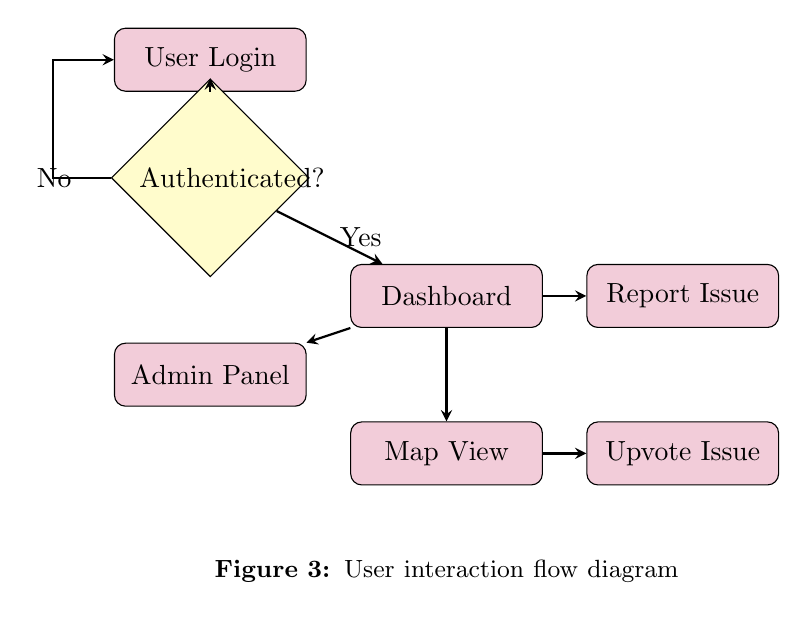
\begin{tikzpicture}[
    node distance=1.8cm,
    state/.style={rectangle, draw=black, fill=purple!20, text width=2.2cm, text centered, rounded corners, minimum height=0.8cm},
    decision/.style={diamond, draw=black, fill=yellow!20, text width=1.8cm, text centered, minimum height=0.8cm},
    arrow/.style={thick,->,>=stealth}
]

% States
\node[state] (login) at (0,4) {User Login};
\node[decision] (auth_check) at (0,2.5) {Authenticated?};
\node[state] (dashboard) at (3,1) {Dashboard};
\node[state] (report) at (6,1) {Report Issue};
\node[state] (map_view) at (3,-1) {Map View};
\node[state] (upvote) at (6,-1) {Upvote Issue};
\node[state] (admin) at (0,0) {Admin Panel};

% Flow
\draw[arrow] (login) -- (auth_check);
\draw[arrow] (auth_check) -- node[right] {Yes} (dashboard);
\draw[arrow] (auth_check) -- node[left] {No} ++(-2,0) |- (login);
\draw[arrow] (dashboard) -- (report);
\draw[arrow] (dashboard) -- (map_view);
\draw[arrow] (map_view) -- (upvote);
\draw[arrow] (dashboard) -- (admin);

\node[text width=8cm, text centered] at (3,-2.5) {\small\textbf{Figure 3:} User interaction flow diagram};

\end{tikzpicture}
\end{figure}

% Technology Stack Diagram
\begin{figure}[h]
\centering
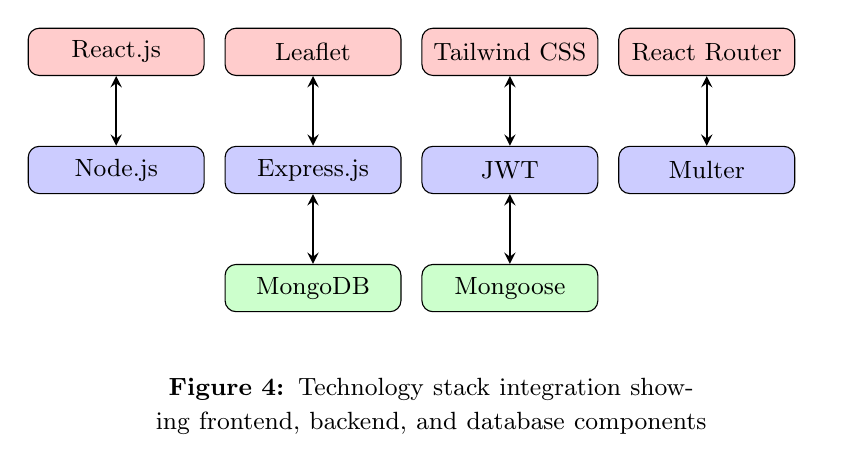
\begin{tikzpicture}[
    node distance=1.2cm,
    tech/.style={rectangle, draw=black, text width=2cm, text centered, rounded corners, minimum height=0.6cm, font=\small},
    frontend_tech/.style={tech, fill=red!20},
    backend_tech/.style={tech, fill=blue!20},
    database_tech/.style={tech, fill=green!20},
    arrow/.style={thick,<->,>=stealth}
]

% Frontend Technologies
\node[frontend_tech] (react) at (0,3) {React.js};
\node[frontend_tech] (leaflet) at (2.5,3) {Leaflet};
\node[frontend_tech] (tailwind) at (5,3) {Tailwind CSS};
\node[frontend_tech] (router) at (7.5,3) {React Router};

% Backend Technologies
\node[backend_tech] (nodejs) at (0,1.5) {Node.js};
\node[backend_tech] (express) at (2.5,1.5) {Express.js};
\node[backend_tech] (jwt) at (5,1.5) {JWT};
\node[backend_tech] (multer) at (7.5,1.5) {Multer};

% Database Technologies
\node[database_tech] (mongodb) at (2.5,0) {MongoDB};
\node[database_tech] (mongoose) at (5,0) {Mongoose};

% Connections
\draw[arrow] (react) -- (nodejs);
\draw[arrow] (leaflet) -- (express);
\draw[arrow] (tailwind) -- (jwt);
\draw[arrow] (router) -- (multer);
\draw[arrow] (express) -- (mongodb);
\draw[arrow] (jwt) -- (mongoose);

\node[text width=10cm, text centered] at (4,-1.5) {\small\textbf{Figure 4:} Technology stack integration showing frontend, backend, and database components};

\end{tikzpicture}
\end{figure}

% Security Architecture
\begin{figure}[h]
\centering
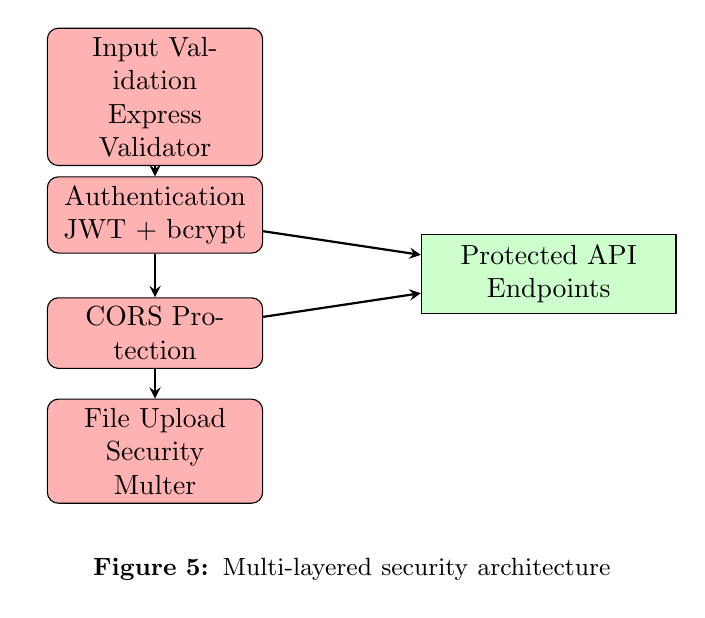
\begin{tikzpicture}[
    node distance=1.5cm,
    security/.style={rectangle, draw=black, fill=red!30, text width=2.5cm, text centered, rounded corners, minimum height=0.8cm},
    arrow/.style={thick,->,>=stealth}
]

% Security Layers
\node[security] (input_val) at (0,3) {Input Validation\\Express Validator};
\node[security] (auth) at (0,1.5) {Authentication\\JWT + bcrypt};
\node[security] (cors) at (0,0) {CORS Protection};
\node[security] (upload) at (0,-1.5) {File Upload Security\\Multer};

% Protected Resources
\node[rectangle, draw=black, fill=green!20, text width=3cm, text centered, minimum height=1cm] (api) at (5,0.75) {Protected API\\Endpoints};

% Connections
\draw[arrow] (input_val) -- (auth);
\draw[arrow] (auth) -- (cors);
\draw[arrow] (cors) -- (upload);
\draw[arrow] (auth) -- (api);
\draw[arrow] (cors) -- (api);

\node[text width=8cm, text centered] at (2.5,-3) {\small\textbf{Figure 5:} Multi-layered security architecture};

\end{tikzpicture}
\end{figure}
